\subsection{ROLLO: Reactor evOLutionary aLgorithm Optimizer}

\begin{frame}
    \frametitle{Research Objectives: AHTR optimization for non-conventional designs}
    \begin{block}{Technical Gap}
      \begin{itemize}
        \item Optimization tools for generating new reactor designs enabled by
        3D printing do not exist
        \item Few demonstrations of reactor optimization for non-conventional 
        geometries and parameters exist
      \end{itemize}
    \end{block}
    \begin{block}{Research Objectives: AHTR optimization for non-conventional designs}
        \begin{itemize}
            \item Develop an open-source tool that enables generative reactor design 
            optimization with evolutionary algorithms 
            \item Demonstrate successful tool application on AHTR optimization for 
            non-conventional reactor geometries and fuel distributions
        \end{itemize}
    \end{block}
  \end{frame}

\begin{frame}
    \frametitle{ROLLO: Reactor evOLutionary aLgorithm Optimizer}
    \begin{figure}
        
\includegraphics[width=0.7\linewidth]{figures/rollo-logo.png} 
        \caption{ROLLO (Reactor evOLutionary aLgorithm Optimizer) logo.}
    \end{figure}
    \begin{itemize}
        \visible<1->{\item ROLLO (Reactor evOLutionary aLgorithm Optimizer) is a Python 
        package that applies evolutionary algorithms to optimize nuclear reactor design}
        \visible<2->{\item ROLLO provides a general genetic algorithm framework, sets up 
        parallelization for the user, and promotes usability with an input file that
        only exposes mandatory parameters}
        \visible<3->{\item Designed to be: effective, flexible, open-source, parallel, 
        reproducible}
    \end{itemize}
\end{frame}

\begin{frame}
    \frametitle{How does ROLLO work?}
    \begin{columns}
        \begin{column}{0.7\textwidth}

            \vspace{-0.5cm}
            ROLLO Flow 
            \begin{itemize}
                \item Reads and validates the JSON input file
                \item Blue blocks 
                \begin{itemize}
                    \item Evolutionary algorithm is driven by \acrfull{DEAP} 
                \end{itemize}
                \item Orange blocks
                \begin{itemize}
                    \item Reactor modeling software evaluates the fitness of each 
                    reactor model in each generation 
                \end{itemize}
            \end{itemize}

            \vspace{0.2cm}
            For each ROLLO optimization simulation, one must \textbf{balance convergence and 
            computational cost}. 

            \vspace{0.2cm}
            ROLLO's purpose is to help the human reactor designer narrow down reactor design 
            search space. The reactor designer uses the \textbf{computational power 
            available}, to \textbf{narrow down the search space} as much as possible.
        \end{column}
        \begin{column}{0.3\textwidth}
            \vspace{-0.3cm}
            \begin{figure}
                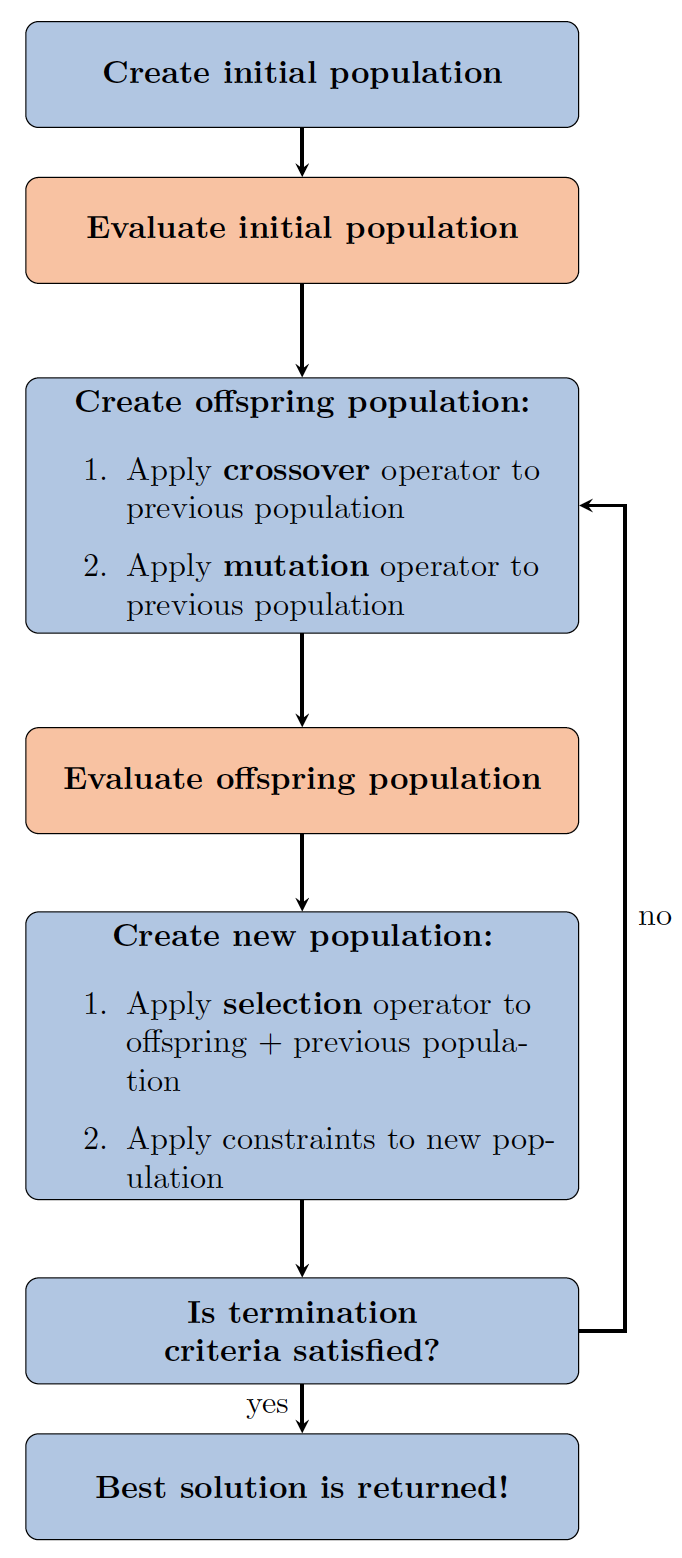
\includegraphics[width=0.97\linewidth]{figures/rollo-flow2.png} 
                %\caption{ROLLO's Genetic Algorithm Flow.}
            \end{figure}
        \end{column}
    \end{columns}
\end{frame}
